\documentclass[final,hyperref={pdfpagelabels=false}]{beamer}

\usepackage[orientation=portrait,size=a0,scale=1.4]{beamerposter} % Use the beamerposter package for laying out the poster with a portrait orientation and an a0 paper size

% \toprule, \midrule, \bottomrule % instead of \hline
\usepackage{booktabs}
% Tables that can fit page length
\usepackage{tabularx}
% Multirows and multicolumns in table
\usepackage{multirow, multicol}

\usetheme{I6pd2} % Use the I6pd2 theme supplied with this template
\usepackage[english]{babel} % English language/hyphenation
\usepackage{amsmath,amsthm,amssymb,latexsym} % For including math equations, theorems, symbols, etc

%\usepackage{times}\usefonttheme{professionalfonts}  % Uncomment to use Times as the main font
%\usefonttheme[onlymath]{serif} % Uncomment to use a Serif font within math environments

%\boldmath % Use bold for everything within the math environment

\graphicspath{{media/}} % Location of the graphics files
\usecaptiontemplate{\small\structure{\insertcaptionname~\insertcaptionnumber:\,}\insertcaption} % A fix for figure numbering
\usepackage{siunitx}
\usepackage{caption}

%set reference on one line
\setbeamertemplate{bibliography entry article}{}
\setbeamertemplate{bibliography entry title}{}
\setbeamertemplate{bibliography entry location}{}
\setbeamertemplate{bibliography entry note}{}

% Acronyms
\usepackage{acronym}
\acrodef{lidar}{Light Detection And Ranging}
\acrodefplural{lidar}{Light Detection And Ranging}
\acrodef{ICP}{Iterative Closest Point}
\acrodef{DOF}{Degrees Of Freedom}
\acrodef{RTS}{Robotic Total Station}
\acrodefplural{RTS}{Robotic Total Stations}
\acrodef{GNSS}{Global Navigation Satellite System}
\acrodef{RTK}{Real Time Kinematics}
\acrodef{GCP}{Ground Control Point}
\acrodef{UAV}{Unmanned Aerial Vehicle}
\acrodef{IQR}{Interquartile Range}
\acrodef{IMU}{Inertial Measurement Unit}
\acrodef{SLAM}{Simultaneous Localization and Mapping}
\acrodef{INS}{Inertial Navigation System}
\acrodef{UGV}{Uncrewed Ground Vehicle}
\acrodef{NTP}{Network Time Protocol}
\acrodef{HD}{High-Definition}
\acrodef{TLS}{Terrestrial Laser Scanner}
\acrodef{CAD}{Computer-Aided Design}
\acrodef{URDF}{Unified Robot Description Format}
\acrodef{RTS-GT}{Robotic Total Stations Ground Truthing dataset}

% models
% \bm % in equations for proper bold font
\usepackage{bm}

%----------------------------------------------------------------------------------------
%	TITLE SECTION 
%----------------------------------------------------------------------------------------

\title{\huge RTS-GT: Robotic Total Stations Ground Truthing dataset} % Poster title

\author{\normalsize Maxime Vaidis$^{1}$, 
Mohsen Hassanzadeh Shahraji$^{1}$, 
Effie Daum$^{1}$, 
\\William Dubois$^{1}$,
Philippe Giguère$^{1}$, 
François Pomerleau$^{1}$} % Author(s)} % Author(s)

\institute{\small$^1$ Northern Robotics Laboratory, Universit\'e Laval} % Institution(s)

%----------------------------------------------------------------------------------------
%	FOOTER TEXT
%----------------------------------------------------------------------------------------

\newcommand{\leftfoot}{IEEE International Conference on Robotics and Automation 2024} % Left footer text

\newcommand{\rightfoot}{\{maxime.vaidis, francois.pomerleau\}@norlab.ulaval.ca} % Right footer text

%----------------------------------------------------------------------------------------

\begin{document}

\addtobeamertemplate{block end}{}{\vspace*{1ex}} % White space under blocks

\begin{frame}[t] % The whole poster is enclosed in one beamer frame

\begin{columns}[t] % The whole poster consists of two major columns, each of which can be subdivided further with another \begin{columns} block - the [t] argument aligns each column's content to the top

\begin{column}{.0125\textwidth}\end{column} % Empty spacer column

\begin{column}{.465\textwidth} % The first column

%----------------------------------------------------------------------------------------
%	OBJECTIVES
%----------------------------------------------------------------------------------------
\vspace{-12.5mm}
\begin{block}{Context \& Motivations}
\begin{itemize}
    \item[\textbf{$\bullet$}] Majority of datasets don't provide the precision and reproducibility of their ground-truth~\cite{KITTI2012, UZH2019};
    \item[\textbf{$\bullet$}] Provide the first dataset to focus on ground truthing done by three \acp{RTS} to obtain the six-\ac{DOF} of robotic platform reference trajectories;
    \item[\textbf{$\bullet$}] Covers a variety of challenging environments collected during \num{17} months in diverse weather conditions, totaling over \num{49} kilometers of trajectories;
    \item[\textbf{$\bullet$}] Precision and the reproducibility of the setups are provided~\cite{Vaidis2023Iros}.
\end{itemize}
\end{block}

\begin{block}{RTS-GT Dataset}
\begin{itemize}
    \item Experimental setup
\end{itemize}
    \vspace{4mm}
    \begin{figure}
        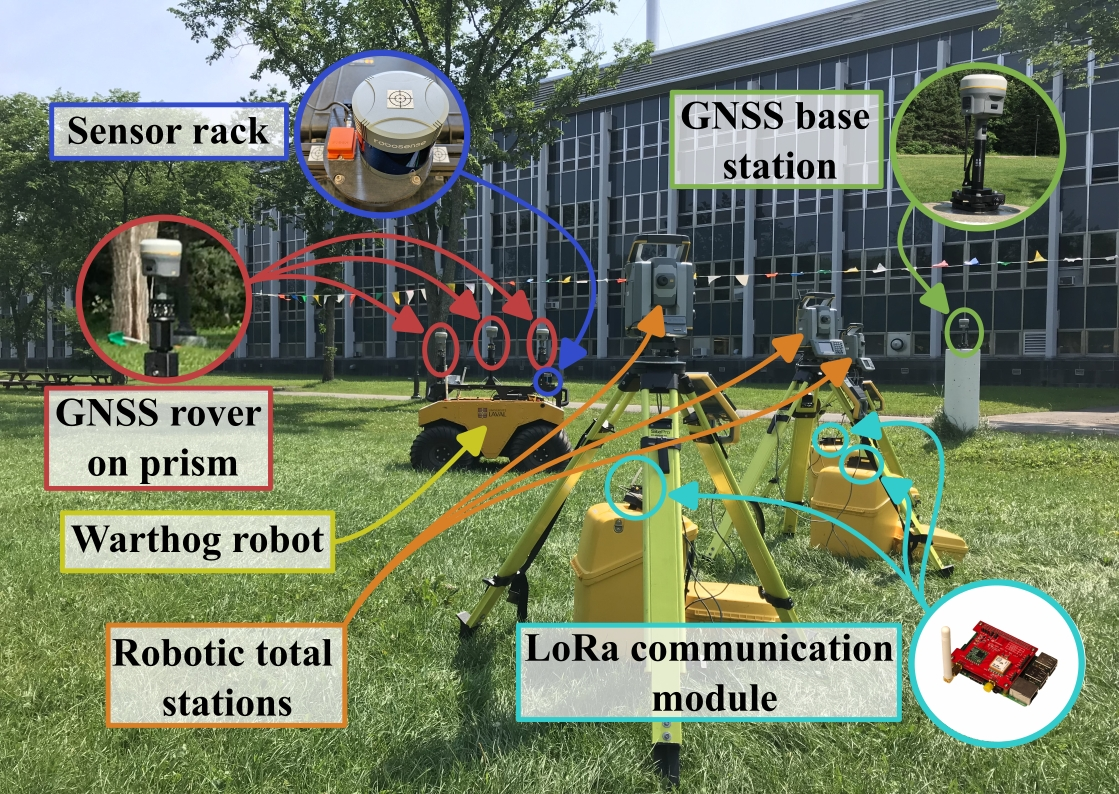
\includegraphics[width=0.735\linewidth]
            {figures/setup.jpg}%
        %\vspace{-7mm}
        \captionsetup{width = 0.975\linewidth, justification=justified, name=Figure 1}
        \caption{
            Setup used on the campus with the Warthog \ac{UGV}. A \ac{GNSS} fixed base station sends corrections to the three \ac{GNSS} rovers on the robot. Three prisms are tracked by three \ac{RTS}. 
            Data are collected by three Raspberry Pi clients connected by USB to the \ac{RTS}. A LoRa communication protocol is used to send data to a Raspberry Pi master located on the \ac{UGV}. The lidar and \ac{IMU} are on the front part of the Warthog.}
        \label{fig:setup_outside}
    \end{figure}
    \vspace{4mm}
    \begin{figure}
        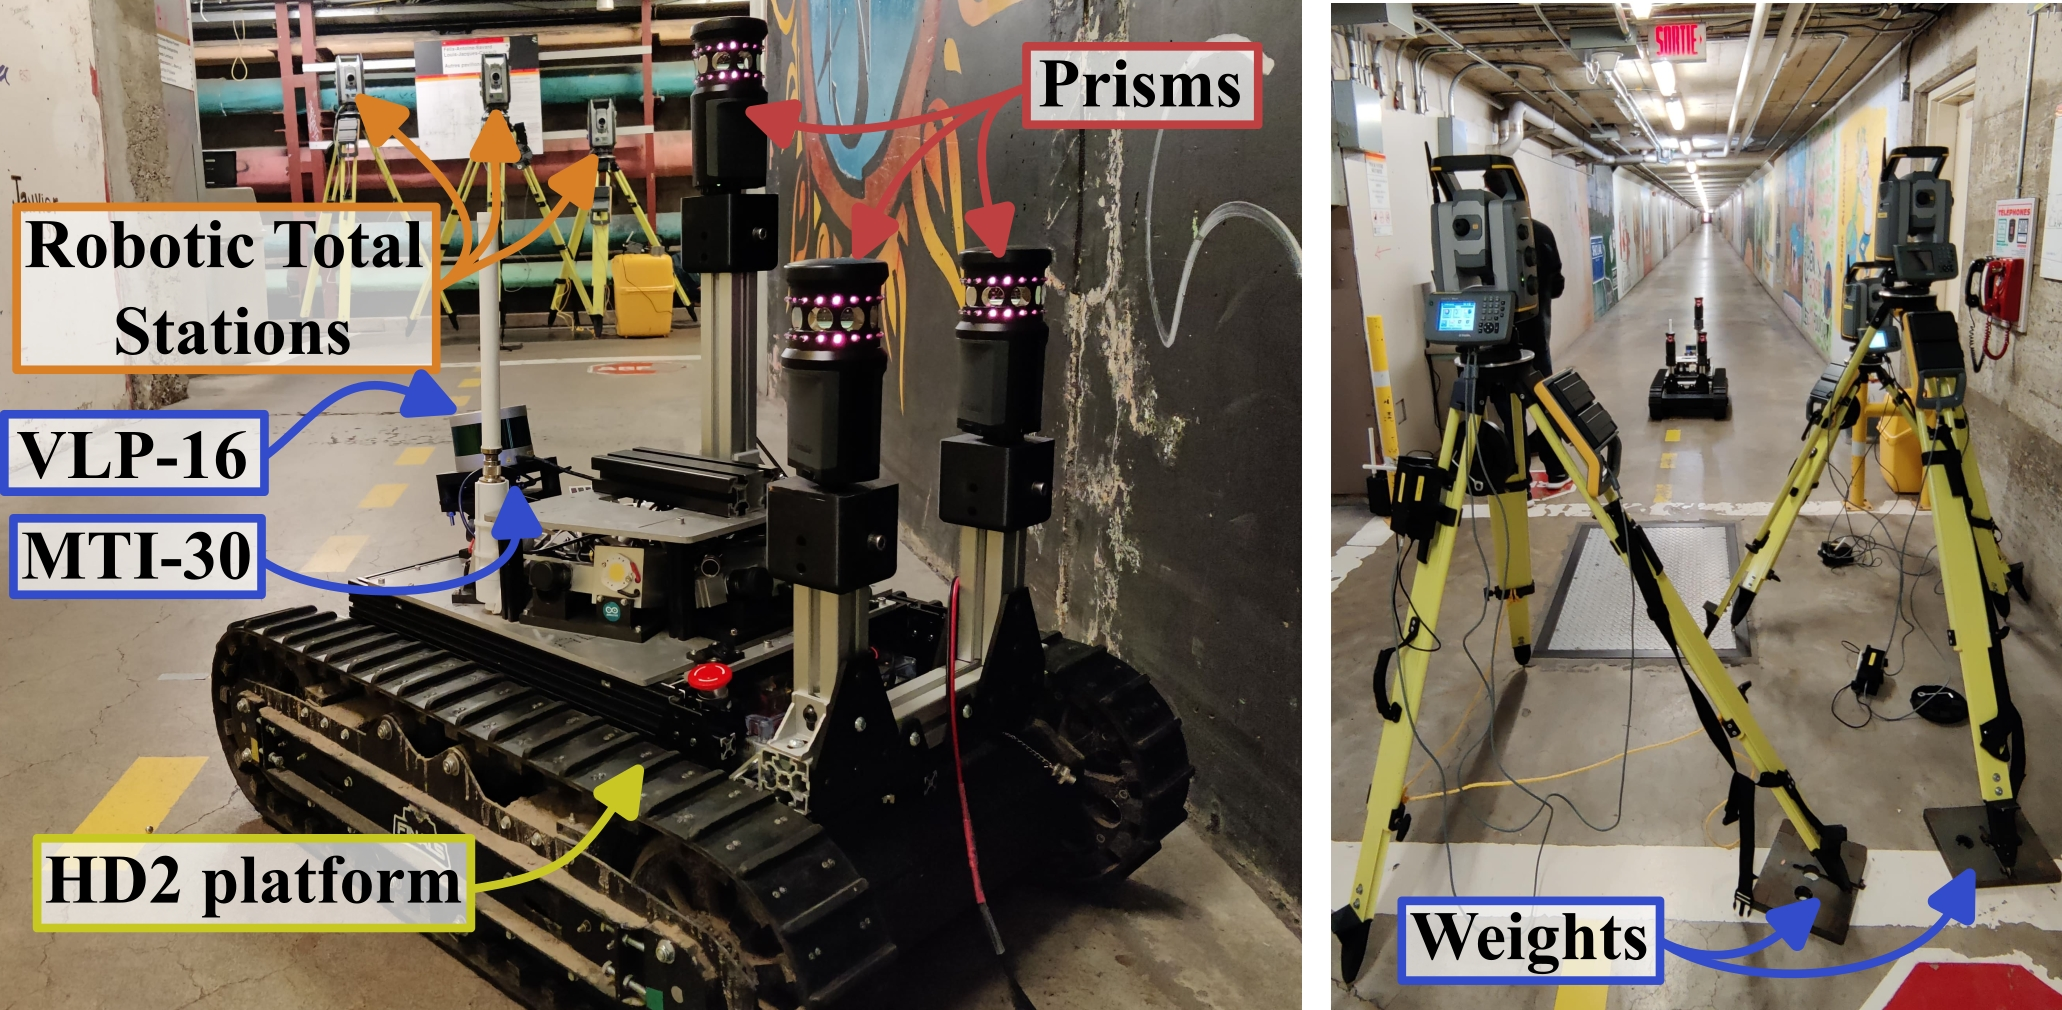
\includegraphics[width=0.82\linewidth]
            {figures/tunnels.jpg}%
        %\vspace{-7mm}
        \captionsetup{width = 0.975\linewidth, justification=justified, name=Figure 2}
        \caption{
            Setup used in the tunnel sites. \emph{Left}: \ac{RTS} setup with the HD2 robot. \emph{Right}: one deployment done in a \SI{120}{\m} tunnel. Because the floor was slippery, heavy weights were added to stabilize the \acp{RTS} tripods.}
        \label{fig:setup_tunnels}
    \end{figure}

\begin{itemize}
    \item Deployments
\end{itemize}
    \vspace{4mm}
    \begin{figure}
        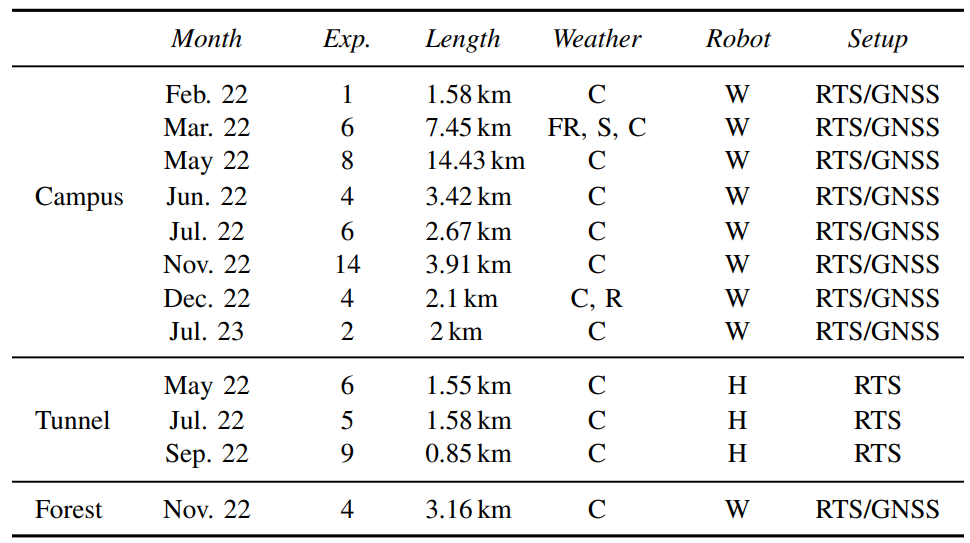
\includegraphics[width=0.72\linewidth]
            {figures/tableau_icra2024_deployment.png}%
        \captionsetup{width = 0.975\linewidth, justification=justified, name=Table 1}
        \caption{
            Table of deployments in the RTS-GT dataset. The weather legend is as follows: C=Clear, FR=Freezing rain, S=Snow, R=Rain. The robot legend means W=Warthog and H=HD2.}
        \label{fig:table_deployment}
    \end{figure}

The deployment sites were on the campus of Université Laval in Quebec City, and its underground tunnels.
This campus comprises buildings, open spaces, and wooded areas.
During these data collection campaigns, various weather conditions were encountered, including clear weather, rain, and even a snowstorm. 
Data from both \ac{RTS} and \ac{GNSS} setups are available for each of the conducted experiments, enabling a comparison of their respective accuracies in generating reference trajectories.
    
\end{block}

%----------------------------------------------------------------------------------------

\end{column} % End of the first column

\begin{column}{.03\textwidth}\end{column} % Empty spacer column
 
\begin{column}{.465\textwidth} % The second column

%----------------------------------------------------------------------------------------
%	New block
%----------------------------------------------------------------------------------------

\vspace{-12.5mm}
\begin{block}{RTS Ground truth protocol}
    \begin{enumerate}
        \item (\SI{30}{\min}) \ac{RTS} units are acclimated to the ambient temperature before data collection can begin;
        \item (\num{5}-\SI{60}{\min}) Tripods for the \ac{RTS} are set up, while the \ac{RTS} units adjust to the ambient temperature;
        \item (\num{10}-\SI{15}{\min}) \ac{RTS} units are mounted on tripods, and we roughly level \ac{RTS} units visually.
        To achieve a finer leveling for \ac{RTS} units, calibrated electronic sensors are utilized;
        \item (\num{3}-\SI{5}{\min}) Raspberry Pi devices are powered on and connected via USB to the \ac{RTS} units to retrieve their data and send it to the master unit for recording. 
        These Raspberry Pi devices also assign a unique prism number to each \ac{RTS} unit to be tracked;
        \item (\num{1}-\SI{2}{\min}) Active prisms are mounted on the \ac{UGV} and powered on with their unique ID.
        To facilitate data processing of multiple experiments conducted by the robots, the same prism ID and positions were adopted during all data acquisition operations;
        \item (\num{1}-\SI{10}{\min}) Verification of proper prism tracking is performed, followed by measurements of static prism positions to enable post-processing extrinsic calibration of \ac{RTS} units.
    \end{enumerate}
\end{block}


\begin{block}{Results}
	
\begin{itemize}
    \item Precision and reproducibility
\end{itemize}
    \vspace{4mm}
    \begin{figure}
        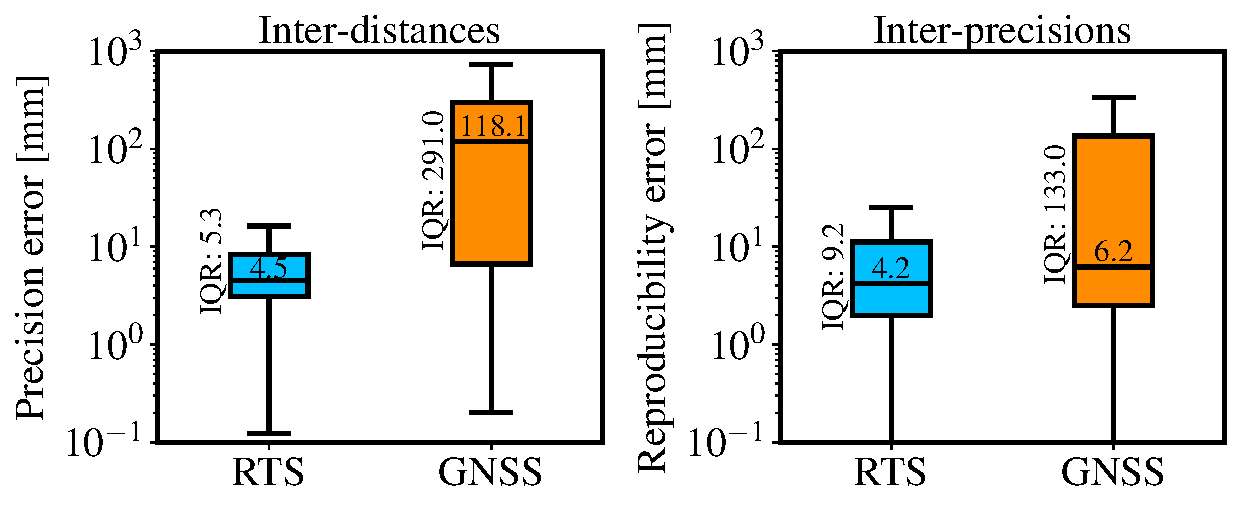
\includegraphics[width=0.7\linewidth]
            {figures/boxplot_inter.pdf}%
        \captionsetup{width = 0.975\linewidth, justification=justified, name=Figure 3}
        \caption{
            Distribution of errors arising for the two setups. \emph{Left}: inter-prism and inter-\ac{GNSS} distances. \emph{Right}: inter-precision distances.
            Results obtained from the \acp{RTS} are denoted in blue, whereas those from the \ac{GNSS} are shown in orange.
            The median error values are in the center of each box, and the \ac{IQR} is indicated alongside for reference.}
        \label{fig:results_precision_reproducibility}
    \end{figure}

\begin{itemize}
    \item Results over different deployments
\end{itemize}
    \vspace{4mm}
    \begin{figure}
        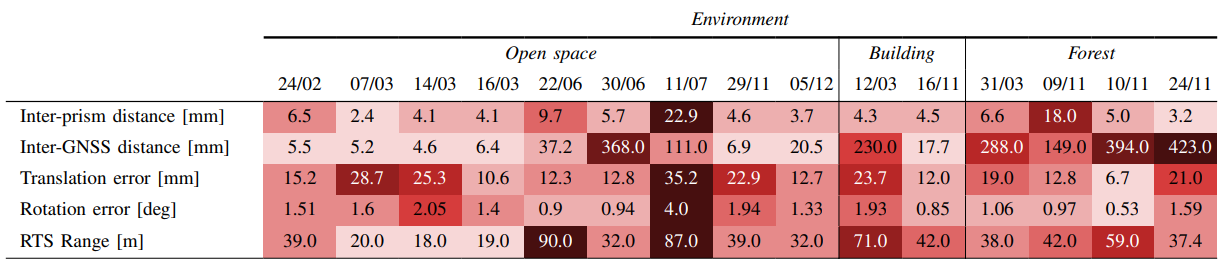
\includegraphics[width=\linewidth]
            {figures/tableau_icra2024_results.png}%
        \captionsetup{width = 0.975\linewidth, justification=justified, name=Table 2}
        \caption{
            Distribution of errors arising for the two setups. \emph{Left}: inter-prism and inter-\ac{GNSS} distances. \emph{Right}: inter-precision distances.
            Results obtained from the \acp{RTS} are denoted in blue, whereas those from the \ac{GNSS} are shown in orange.
            The median error values are in the center of each box, and the \ac{IQR} is indicated alongside for reference.}
        \label{fig:results}
    \end{figure}

\begin{itemize}
    \item Example of trajectories obtained
\end{itemize}
    \begin{figure}
        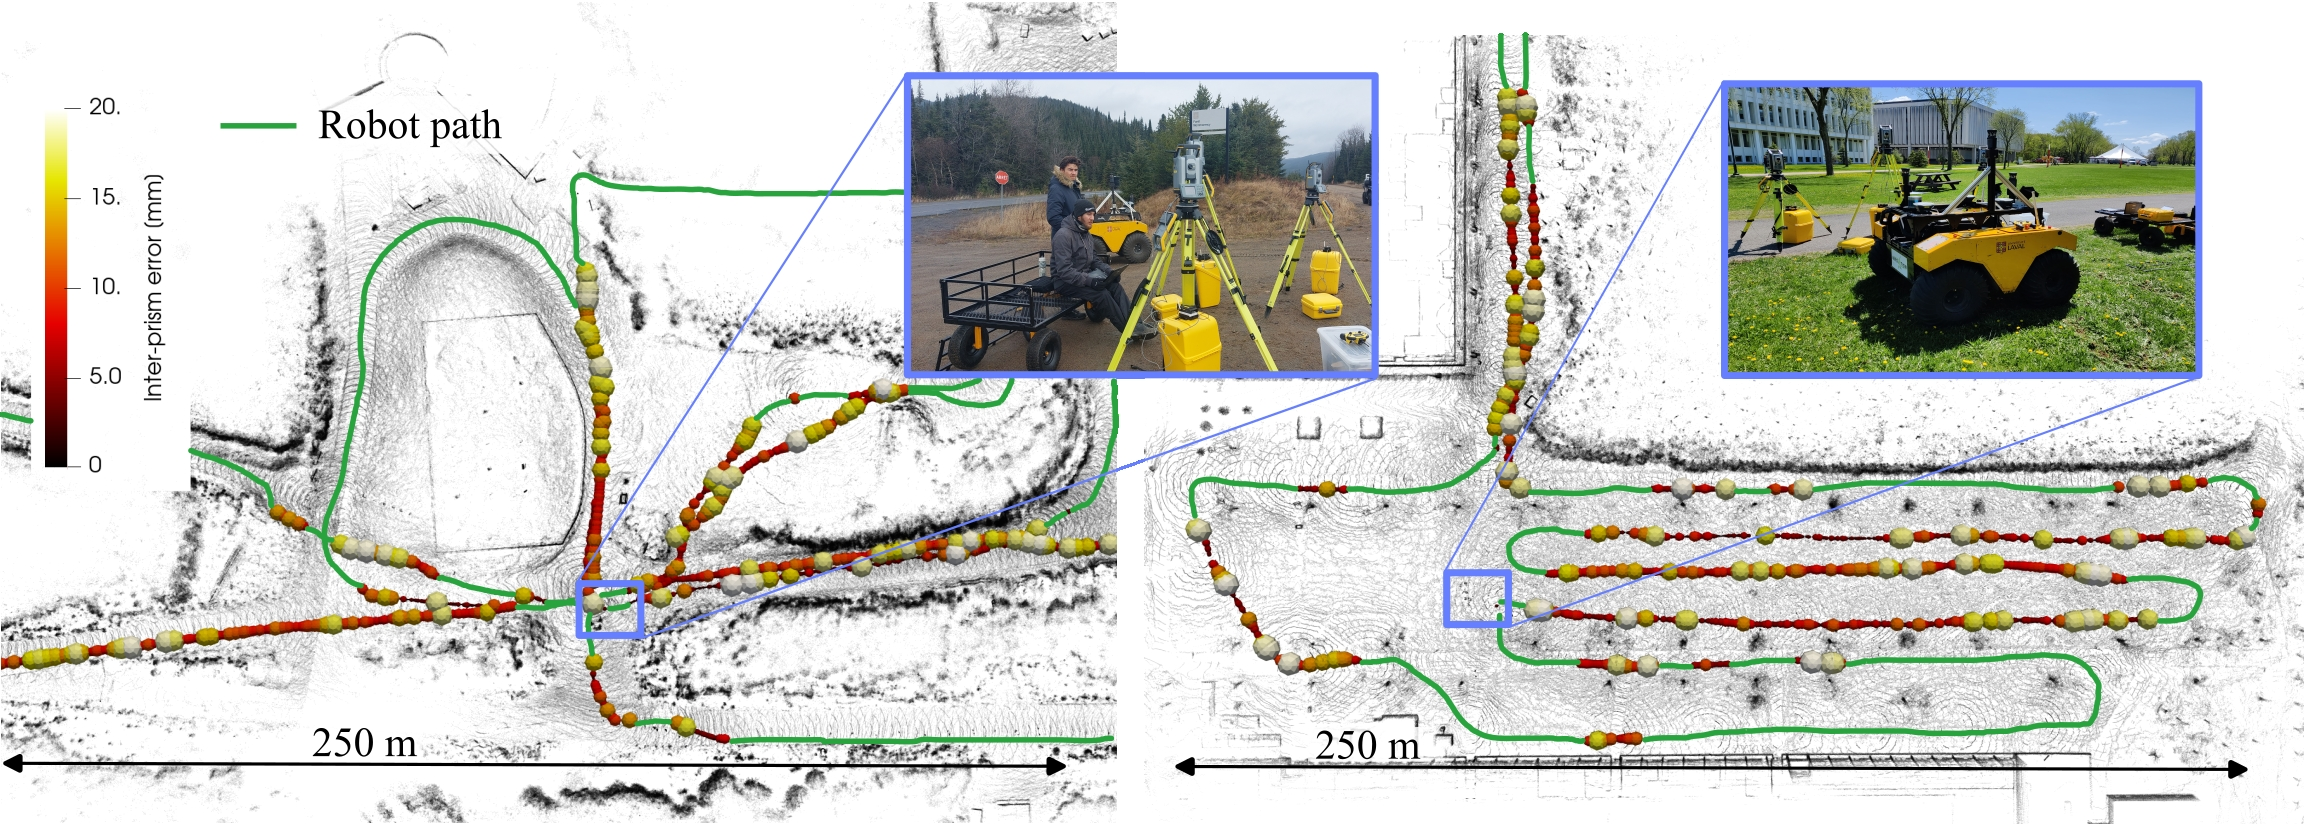
\includegraphics[width=\linewidth]
            {figures/figure_intro.jpg}%
        \captionsetup{width = 0.975\linewidth, justification=justified, name=Figure 4}
        \caption{
            Example of two areas provided in the dataset (bird's-eye view). \emph{Left:} a forest. \emph{Right:} a park on a campus.
            Maps in black are based on lidar scans, while the colored spheres represent the scaled-up uncertainty of the provided ground truth in millimeters.  
            A Clearpath Warthog platform was used during these experiments, whose paths are illustrated in green.}
        \label{fig:setup_outside}
    \end{figure}
	
\end{block}

%----------------------------------------------------------------------------------------
%	ACKNOWLEDGEMENTS
%----------------------------------------------------------------------------------------


\begin{block}{References}
	\footnotesize%
	%\noindent This research was supported by the  Natural  Sciences and Engineering  Research  Council of  Canada  (NSERC)  through the grant CRDPJ 527642-18 SNOW (Self-driving Navigation Optimized for Winter).
	%\vspace{-5mm}
	%\nocite{*} % Insert publications even if they are not cited in the poster
	\bibliographystyle{unsrt}%
	{\footnotesize\bibliography{biblio}}
	%\vspace{-3mm}
\end{block}



%----------------------------------------------------------------------------------------
%	CONTACT INFORMATION
%----------------------------------------------------------------------------------------
%
%\setbeamercolor{block title}{fg=black,bg=orange!70} % Change the block title color
%
%\begin{block}{Contact Information}
%
%\begin{itemize}
%\item Web: \href{http://www.university.edu/smithlab}{http://www.university.edu/smithlab}
%\item Email: \href{mailto:john@smith.com}{john@smith.com}
%\item Phone: +1 (000) 111 1111
%\end{itemize}
%
%\end{block}

%----------------------------------------------------------------------------------------

\end{column} % End of the second column

\begin{column}{.015\textwidth}\end{column} % Empty spacer column
\end{columns} % End of all the columns in the poster
%----------------------------------------------------------------------------------------
%	REFERENCES
%----------------------------------------------------------------------------------------
%
%\begin{block}{References}
%\vspace{-5mm}
%\nocite{*} % Insert publications even if they are not cited in the poster
%\bibliographystyle{unsrt}%
%{\small\bibliography{biblio}}
%\vspace{-3mm}
%\end{block}

\end{frame} % End of the enclosing frame

\end{document}